\section{The Measurement}
\subsection{What are we measuring}
\subsection{How are we measuring it}
\subsection{Run Plan}

\section{The Apparatus}
\subsection{Hall A HRS Spectrometers}
\subsection{CEBAF Accelerator}

% \chapter{\bf{Chapter 2 Title}    % Chapter  2
%Introductory paragraph of Chapter 2.......
%
%\section{First section Title}
%
%First section text......
%
%
%
%\subsection{First Subsection Title}
%
%
%The cross section for elastic electron scattering from the spin one-half
%$^3$H  nucleus is given, in the one-photon exchange approximation, by:
%\beqn
%{  {d\sigma} \over {d\Omega} } (E,\Theta)  =
%{  {(Z\alpha)^2 E^\prime} \over {4 E^3  \sin^4 \left( {\Theta \over 2} \right)}  }
%\left[ A(Q^2) \cos^2 \left( {\Theta \over 2} \right) +
%B(Q^2) \sin^2 \left( {\Theta \over 2} \right) \right],
%\label{morefequ}
%\eeqn
%where $Z$ is the nuclear charge, $\alpha$ is the fine-structure constant,
%$E$ and $E'$ are the incident and scattered electron energies,
%$\Theta$ is the electron scattering angle, $Q^2 = 4 E E' \sin^2 (\Theta/2)$ is
%minus the squared four-momentum transfer,
%and $A(Q^2)$ and $B(Q^2)$ are the $^3$H elastic structure functions, given in
%terms of the charge and magnetic form factors as:
%\beqn
%{   A(Q^2) = {   { F^2_C(Q^2) +
%(1+\kappa)^2 \tau F^2_M(Q^2) } \over {1 + \tau} }    },
%\label{more1}
%\eeqn
%\beqn
%{ B(Q^2) =  2 \tau (1+\kappa)^2 F^2_M(Q^2) },
%\label{more2}
%\eeqn
%where
%$\tau=Q^2/4M^2$ with $M$ being the mass of the target nucleus, and
%$\kappa$ is the anomalous magnetic moment of the nucleus.
%
%Here is a reference ~\cite{mara} which needs to be defined in the bibliography.tex file first.
%
%
%Here comes a Figure....
%
% \begin{figure}[!htbp]
%  \begin{center}
%    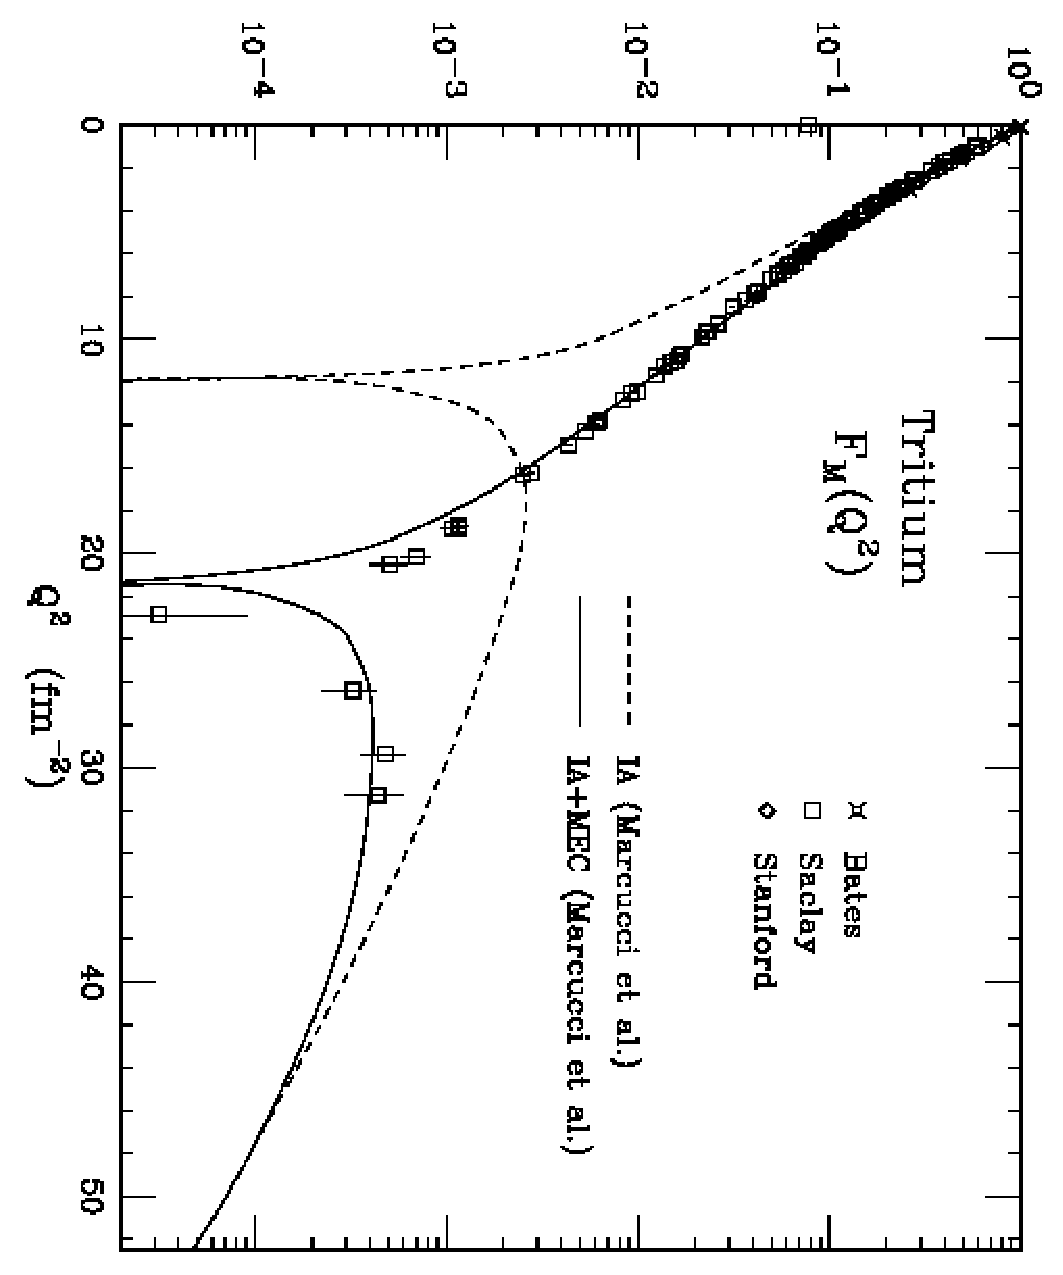
\includegraphics[angle=90, scale=0.65]{./chap2-exp/fig/tritium_past.eps}
%  \end{center}
%  \caption[Tritium Magnetic Form Factor Past Data]{
%    \footnotesize Tritium Mag. Form Factor past data.
%  }
%  \label{fig:TritiumM}
%\end{figure}
%
%Use the label name to refer to  Figure  ~\ref{fig:TritiumM}.
%
%
%\subsection{Second Subsection  Title}
%
%Subsection text..........
%
%
%
%\subsubsection{First Subsubsection}
%
%This is a subsubsection.
%
%
%
%\subsubsection{Second Subsubsection}
%
%This another  subsubsection.

\section{Beamline Components}
\setcounter{figure}{0}
\setcounter{table}{0}
\setcounter{equation}{0}
Here I am talking about the raster and how friggin awesome it is.

\begin{figure}
	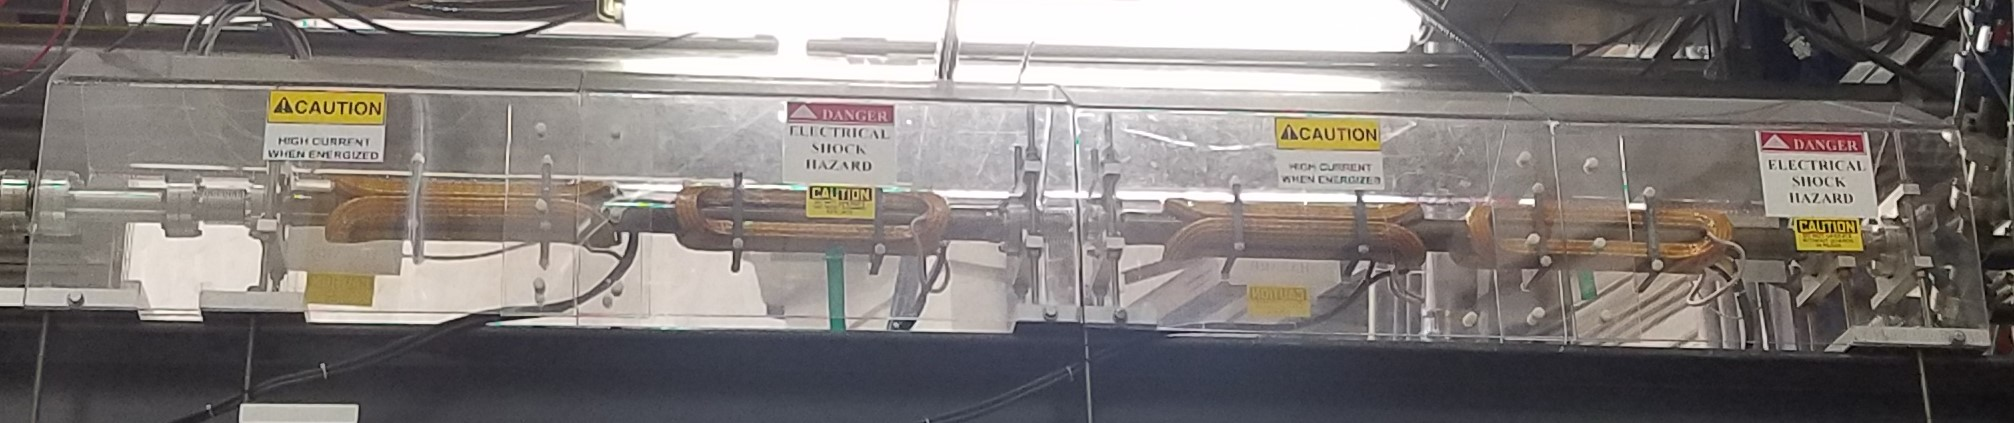
\includegraphics[width=\linewidth]{./chap2-exp/fig/raster_pic.jpg}
	\caption{The Hall A raster consists of four dipole magnets on the beamline}
	\label{fig:raster}
\end{figure}

The raster is a beamline apparatus in Hall A for spreading the beam onto the target, rather than being at a single point. This is done to prevent localized heating of the target. The raster consists of four dipole magnets, two for steering in the x-direction and two for steering in the y-direction.

Each raster magnet is powered by a triangle wave of approximately 25kHz. \textbf{When running properly, the x-direction magnets will be synced and the y-direction magnets will be synced. FIX SENTENCE FOR REDUNDANCY.} This syncing ensures that the magnets are always working together to create the desired beam spread.

\begin{figure}
	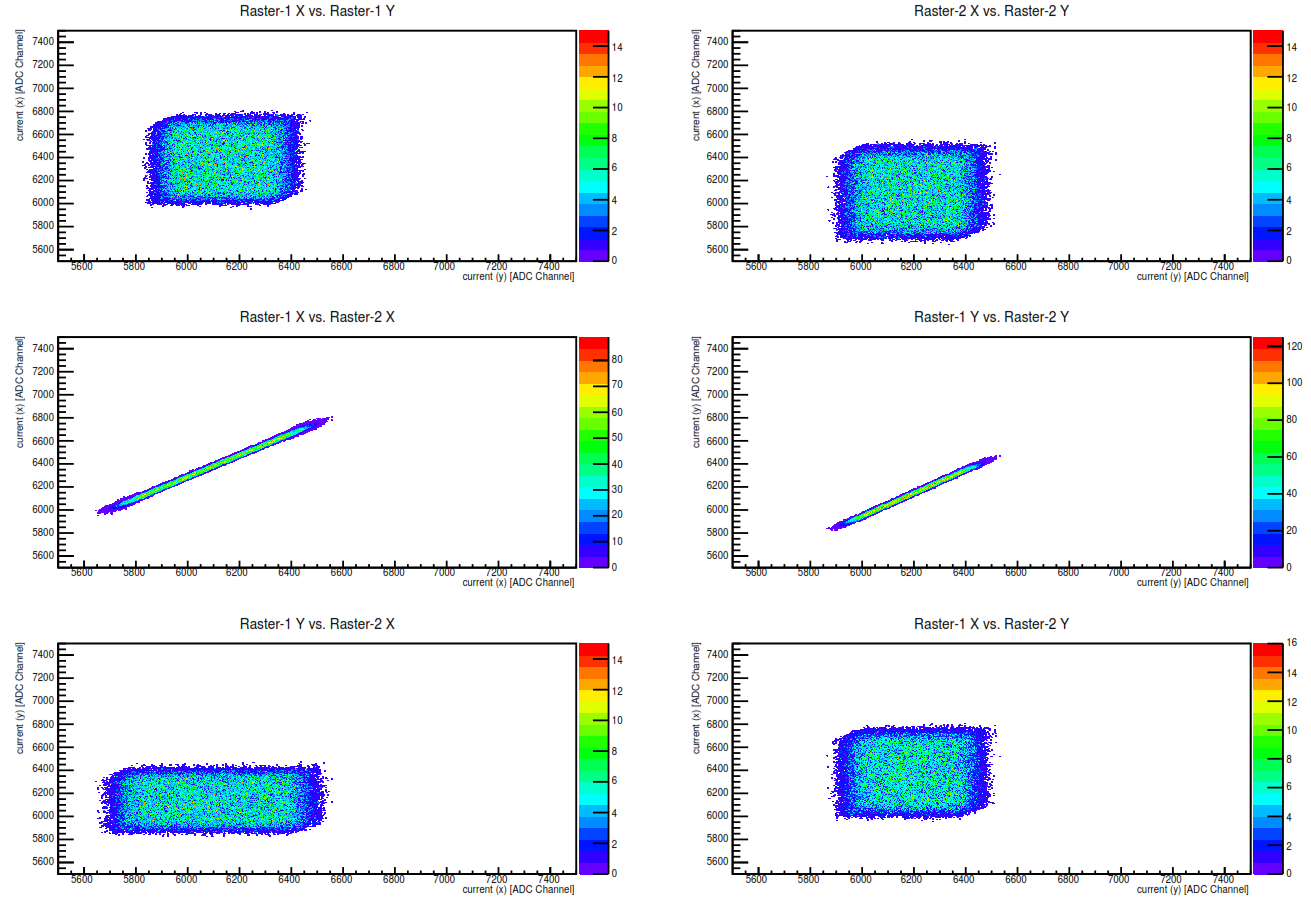
\includegraphics[width=\linewidth]{./chap2-exp/fig/raster_sync.png}
	\caption{The X and Y raster pairs are each synced to produce the maximum kick. The X and Y directions are uncorrelated so that the beam travels uniformly over the target.}
	\label{fig:raster}
\end{figure}
